% Created 2019-04-23 Tue 22:27
% Intended LaTeX compiler: pdflatex
\documentclass[11pt]{article}
\usepackage[utf8]{inputenc}
\usepackage[T1]{fontenc}
\usepackage{graphicx}
\usepackage{grffile}
\usepackage{longtable}
\usepackage{wrapfig}
\usepackage{rotating}
\usepackage[normalem]{ulem}
\usepackage{amsmath}
\usepackage{textcomp}
\usepackage{amssymb}
\usepackage{capt-of}
\usepackage{hyperref}
\author{Kai Lukowiak}
\date{\today}
\title{}
\hypersetup{
 pdfauthor={Kai Lukowiak},
 pdftitle={},
 pdfkeywords={},
 pdfsubject={},
 pdfcreator={Emacs 26.2 (Org mode 9.1.9)},
 pdflang={English}}
\begin{document}

\tableofcontents

\section{Org Mode Python}
\label{sec:org644b27f}

Obviously ever thing is better in Emacs. With a bit of setup, \href{https://github.com/gregsexton/ob-ipython}{found here}, it is
possible to have plain text, org style formatting and, evaluated code, and images
at the tips of your finger.

\subsection{Benefits:}
\label{sec:orgdcdc452}
\begin{itemize}
\item Org-mode is highly extensible
\item Auto complete, pep8 and other options are available
\item Git integration is far easier
\end{itemize}


\subsection{Limitations}
\label{sec:org2a0b1f1}
\begin{itemize}
\item Messy interactive graphs
\item Hard to set up
\item Vim users look at you weird
\end{itemize}

\subsection{Examples:}
\label{sec:orgc798505}

\begin{verbatim}
import matplotlib.pyplot as plt
import numpy as np
\end{verbatim}

\begin{verbatim}
%matplotlib inline
plt.hist(np.random.randn(20000), bins=200);
\end{verbatim}

\begin{center}
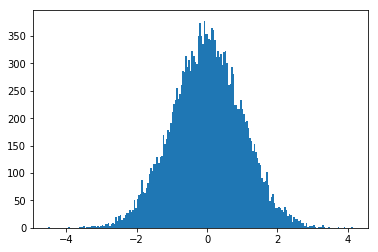
\includegraphics[width=.9\linewidth]{./obipy-resources/RDLupI.png}
\end{center}

It is trivial to mix code and analysis.

\begin{verbatim}
def foo(x):
    return x + 9

[foo(x) + 7 for x in range(7)]
\end{verbatim}

\begin{verbatim}
[16, 17, 18, 19, 20, 21, 22]
\end{verbatim}



\subsubsection{Issues:}
\label{sec:org9d98de1}
Care must be taken to name code chunks

\begin{verbatim}
try:
   foo(1)
except :  print("Did not work")
\end{verbatim}



This one is named correctly.

\begin{verbatim}
foo(4)
print("did work")
\end{verbatim}

My current setup after getting a new laptop is subpar, still check it out.
\end{document}
